\documentclass{article}

\usepackage[margin=1.0in]{geometry}
\usepackage{graphicx}
\usepackage{amsmath}
\usepackage{float}
\usepackage{enumitem}
\usepackage{gensymb}

\title{CSC 577 HW6}
\date{2/27/2019}
\author{Simon Swenson}

\begin{document}

\pagenumbering{gobble}
\maketitle
\pagenumbering{arabic}

\section{Introduction}

We explored using lighting data to recover surface normals and albedo in this 
assignment. The first part was a straightforward application of what we learned 
in class. The second part (graduate portion) was a little more tricky. If the 
image were only lit by three lights, pure blue, pure red, and pure green, it 
would be straightforward to separate the image into its three channels, and 
assign each channel to each light. However, we have multiple lights. We use a 
weighted sum to find an equivalent pure red light, pure green light, and pure 
blue light.

\section{Standard Normal Vector Recovery and Surface Reconstruction}

\begin{figure}[!ht]
	\centering
	
\includegraphics[width=80mm]{figs/4-1.png}
	\caption{An representative of the input images. Just from this image, my 
        brain infers a checkered albido and four extrema, one at the center of 
        each quadrant. The diagonals are the same extrema. This gives us a 
        fuzzy target which we can use to check the results of our algorithm 
        later on.}
\end{figure}

\subsection{Recovering Normal Vectors}

Before we can attempt this problem, we need to make several assumptions to 
simplify the math. First of all, we assume the surface is lambertian. That is, 
its shading is directly proportional to the dot product between the light 
direction and the surface. Second, we assume there are no \textit{hard} shadows. 
Hard shadows make the task of finding normals difficult, because we must exclude 
the corresponding light when we solve for that pixel's normal. Instead, no hard 
shadows means we can treat each pixel uniformly without having to check for 
this.

Recall that, at a given pixel, to generate the intensity for that pixel from a 
given light and surface normal, we simply dot the two together (and multiply by 
the albedo). Thus, we have the equation:

$$
I_i(x, y) = V_i n
$$

If we have multiple lights and multiple output images, we can rewrite the above 
equation as a matrix equation:

$$
i = V n
$$

where $i$ is a vector of intensities at a pixel value, call the pixel $(x, y)$, 
$V$ is a matrix where each row is a light direction, and $n$ is the surface 
normal, for which we're attempting to solve. Note that, in our case, we have 
seven input images (and seven corresponding lights). This means that $V$ is not 
square, and a unique inverse does not exist. We turn to the non-homogeneous 
least squares method of using the pseudoinverse to compute the solution:

$$
n = (V^T V)^{-1} V^T i
$$

Note that this must be done \textit{for each pixel}. Doing so yields favorable 
results (shown nearby) when showing the surface with respect to a test light 
at (0, 0, 1).

\begin{figure}[!ht]
	\centering
	
\includegraphics[width=80mm]{figs/q1_test_light_output.png}
	\caption{The recovered normals multiplied by a test light at (0, 0, 1). 
        Here, we discard the albedo values. Initially, the strange diagonal 
        pattern does not seem to match our intuition about the surface. However, 
        the intuitive shape described above necessarily has saddle points at at 
        diagonals between the four extrema, yielding the daigonal checkerboard 
        pattern.}
\end{figure}

In addition to recovering the normals, we have also recovered the albedo, which 
is encoded in the length of the normal vectors. The recovered albedo matches our 
intuitive notion above,

\begin{figure}[!ht]
	\centering
	
\includegraphics[width=80mm]{figs/q1_albedo.png}
	\caption{The recovered albedo. A checkerboard pattern, as expected.}
\end{figure}

Finally, we can display the results of the test light at (0, 0, 1) with the 
albedo, which, again, matches our intuition:

\begin{figure}[!ht]
	\centering
	
\includegraphics[width=80mm]{figs/q1_test_light_albedo_output.png}
	\caption{The recovered albedo with the test light at (0, 0, 1) applied.}
\end{figure}

\subsection{Recovering the Surface}

If we assume that the surface is continuous, we can recover the surface from 
the normals. Essentially, the problem boils down to recovering the distance 
(depth, z-value) at every pixel. Recall that, if we have the slope of the 
distance formula, we can recover the actual distance by integrating over a path. 
Thus, if we can recover the instantaneous slope (in x and y directions) at each 
pixel, we can discretely integrate (sum) over a path to recover 
the distance. It turns out that the surface normals encode just that: the 
instantaneous slope. In the x direction:

$$
f_x = -\frac{n_x}{n_z}
$$

and in the y direction:

$$
f_y = -\frac{n_y}{n_z}
$$

All that's left to do at this point is to integrate over a path for each pixel. 
For pixels not in the first row and not in the first column, I opted to take the 
value of the pixel diagonally above and to the left and add both the 
instantaneous x slope and y slope. I felt that using both of these would give me 
better results than only integrating in one direction. However, this cannot 
be done for the first row or first column (or top-left pixel). I assume that the 
top-left pixel has a z coordinate of 0, then, for the first row, I integrate 
only in the x direction from the previous pixels in the row. Similar for the 
first column and y direction. The results show that the surface is indeed very 
close to our initial intuitive guess of it.

\begin{figure}[!ht]
	\centering
	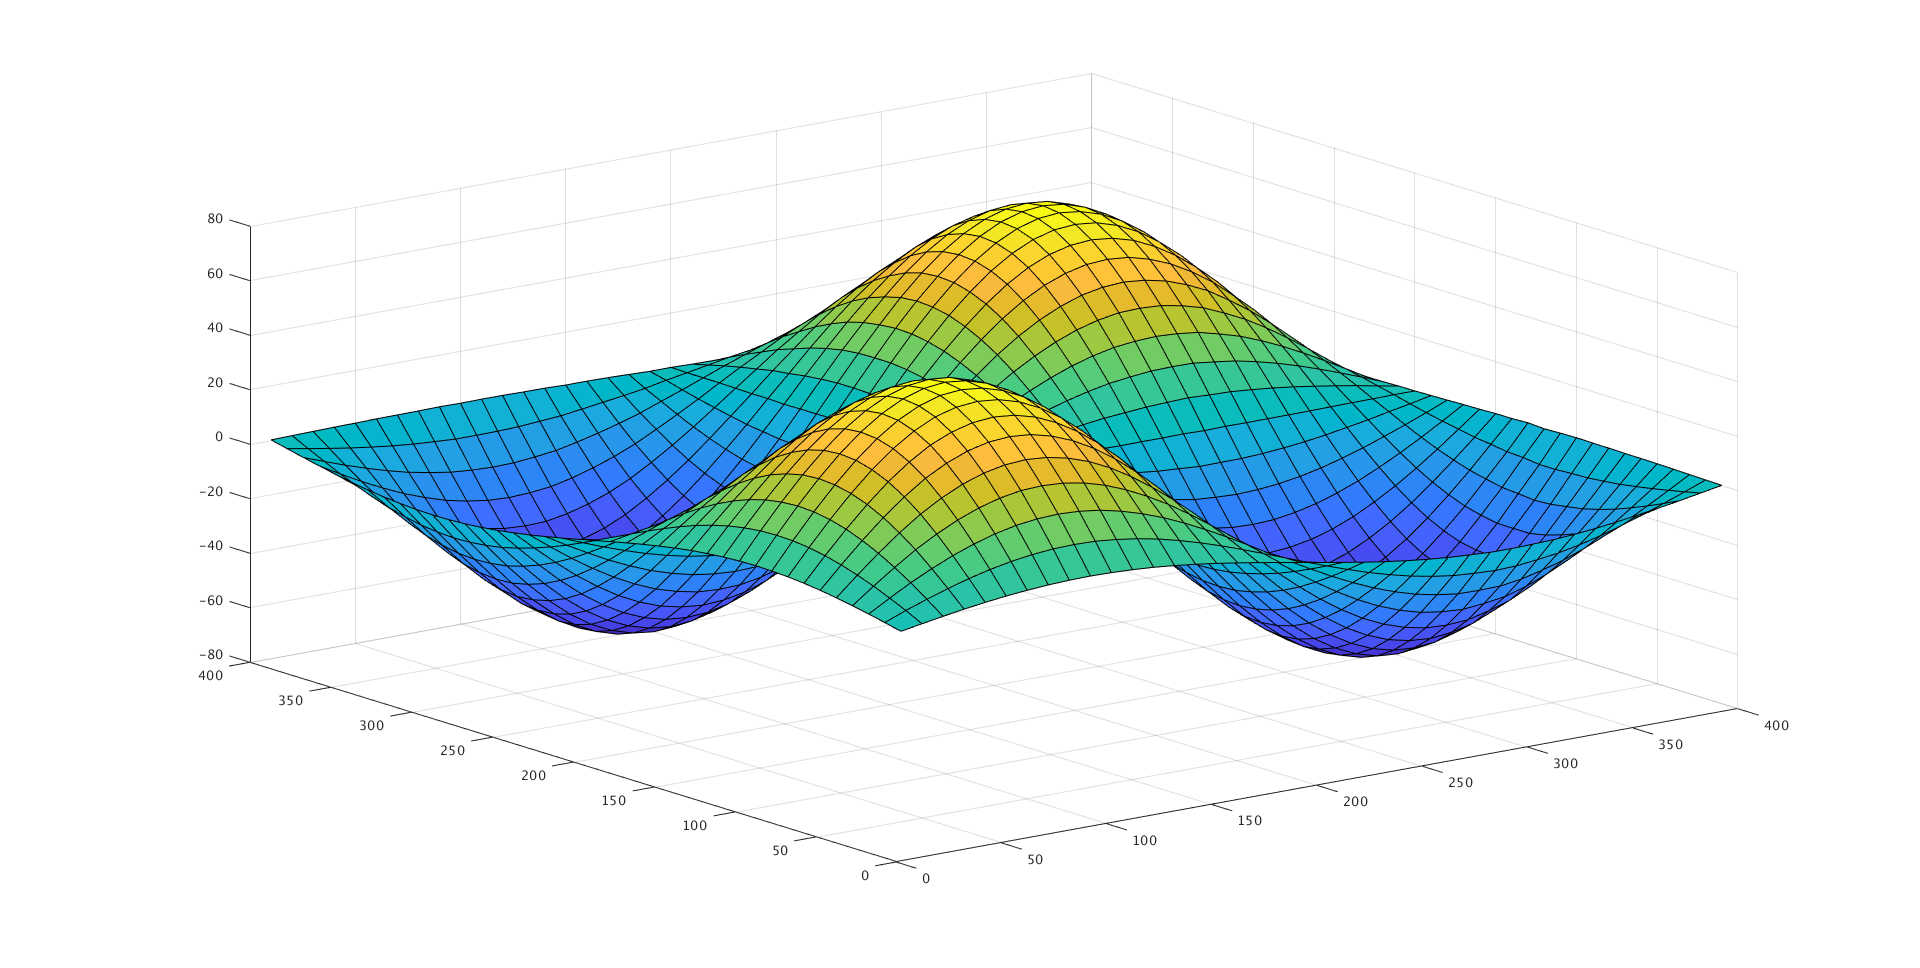
\includegraphics[width=80mm]{figs/q1_surface_plot.png}
	\caption{The recovered surface.}
\end{figure}

\section{Multi-colored Normal Recovery and Surface Reconstruction}

A similar problem is recovering normals and the surface from a single, 
multi-colored image. Here, we need to make some different assumptions, however. 
First, we assume that we not only know the light directions, but also the light 
intensities for each of the three color channels (red, green, blue). In addition, 
we assume that the albedo is constant white.

\begin{figure}[!ht]
	\centering
	
\includegraphics[width=80mm]{figs/color_photometric_stereo_2.png}
	\caption{A multi-colored photometric stereo problem. The surface shape 
        is the exact same as that of the first problem, so I decided to start 
        with this one so that we can compare our results with the results 
        above.}
\end{figure}

\subsection{The First Attempt: Weighted Average of Light Directions}

While it appears that we only have one image to work with, we actually have 
three channels of data: red, green, blue. We could think of these channels as 
representing the surface when illuminated from a pure red light, a pure green 
light, and a pure blue light. However, at this point, we have no idea where 
these theoretical lights would be. Here, we exploit the linearity of light. 
Since the original image is illuminated by five lights (with five known 
directions), we can recover the theoretical, pure red, pure green, and pure blue 
light directions by a linear equation, a weighted sum of the lights, with 
weight based on the normalized intensity of the light for a given channel. This 
yields 3 lights, which we can simply invert to solve for n:

$$
n = V^{-1} i
$$

Our results are not as expected, though, and the output of the raw albedo shows 
why: the recovered albedo is not constant white.

\begin{figure}[!ht]
	\centering
	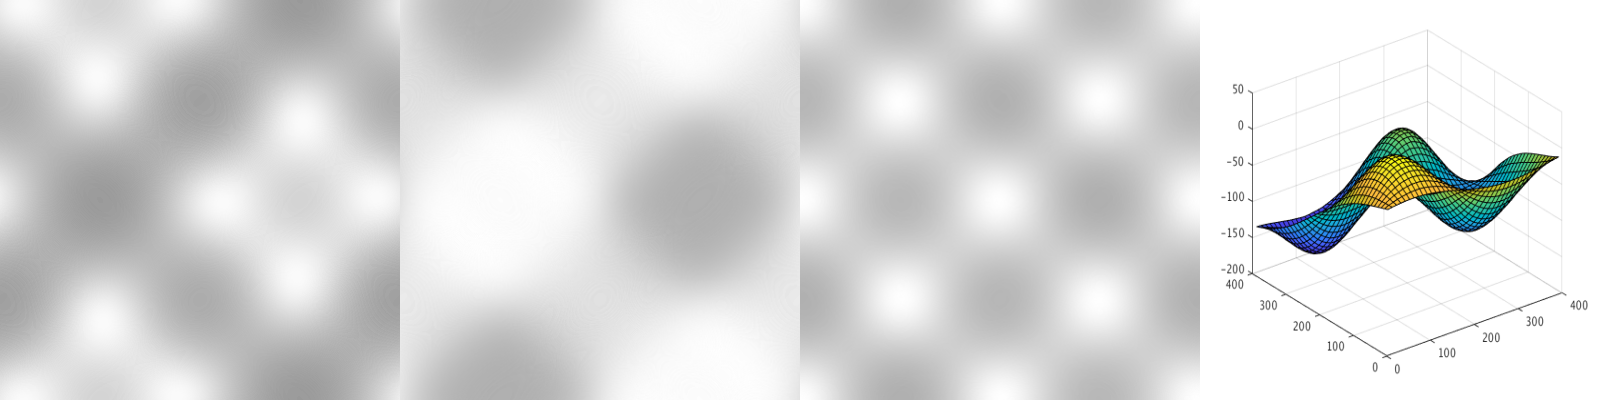
\includegraphics[width=160mm]{figs/q2_im2_bad1_all_figs.png}
	\caption{BAD ATTEMPT 1: Left: Unit normals with test light at (0, 0, 1). Center-left: 
        Recovered albedo. Center-right: Recovered normals with test light at (0, 
        0, 1) (Non-unit normals take albedo into account.) Right: Surface plot. 
        Examining the recovered albedo immediately shows why we are not getting 
        the correct result: We have not constrained the albedo to be constant 
        white. Interestingly, the render which takes the albedo into account 
        looks correct, though. Finally, the plot looks funky, and slopes 
        downward on the left.}
\end{figure}

\subsection{The Second Attempt: Homogeneous Least Squared Error}

At this point, our method seems correct, except that it does not constrain the 
normals to be units. One solution that I considered next was homogeneous least 
squared error, since it constrains the resultant vectors to be units. To attempt 
this, for each pixel, we concatenate the pixel intensities 
to the light positions matrix, then we multiply that matrix by its transpose and 
find the eigenvector with the smallest eigenvalue. However, the results are not 
good.

\begin{figure}[!ht]
	\centering
	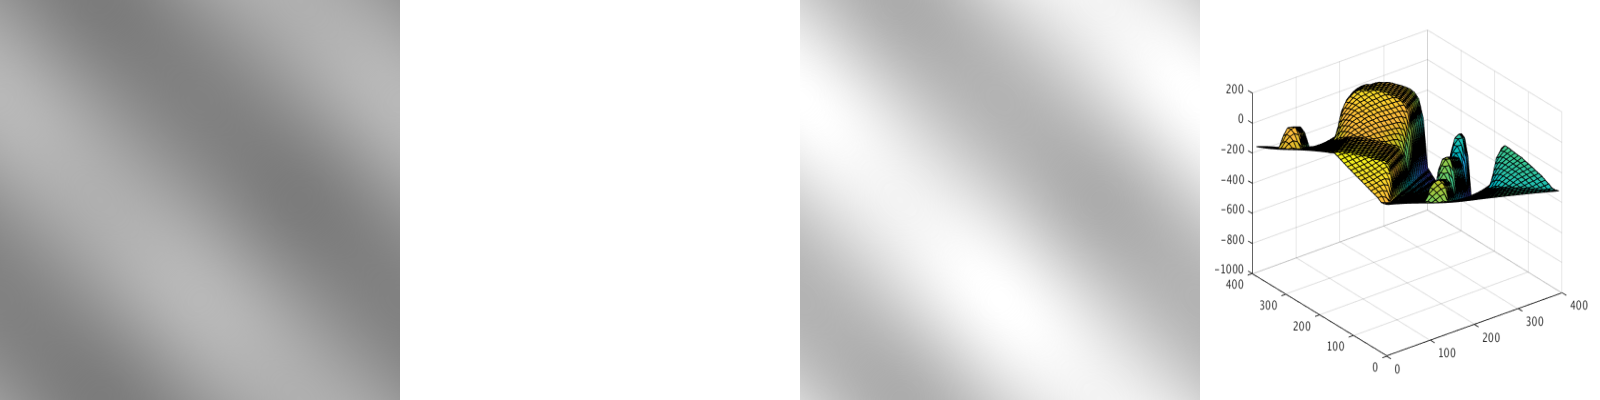
\includegraphics[width=160mm]{figs/q2_im2_bad2_all_figs.png}
	\caption{BAD ATTEMPT 2: Left: Unit normals with test light at (0, 0, 1). Center-left: 
        Recovered albedo. Center-right: Recovered normals with test light at (0, 
        0, 1) (Non-unit normals take albedo into account.) Right: Surface plot. 
        These results do not look right at all! Maybe homogeneous least squared 
        error is not the right path to the solution.}
\end{figure}

\subsection{The Third Attempt: HLSE after Subtracting Means}

One problem we made in the second attempt is that we did not subtract the mean 
values of each column off of the matrix. Doing so results in an even funkier 
image.

\begin{figure}[!ht]
	\centering
	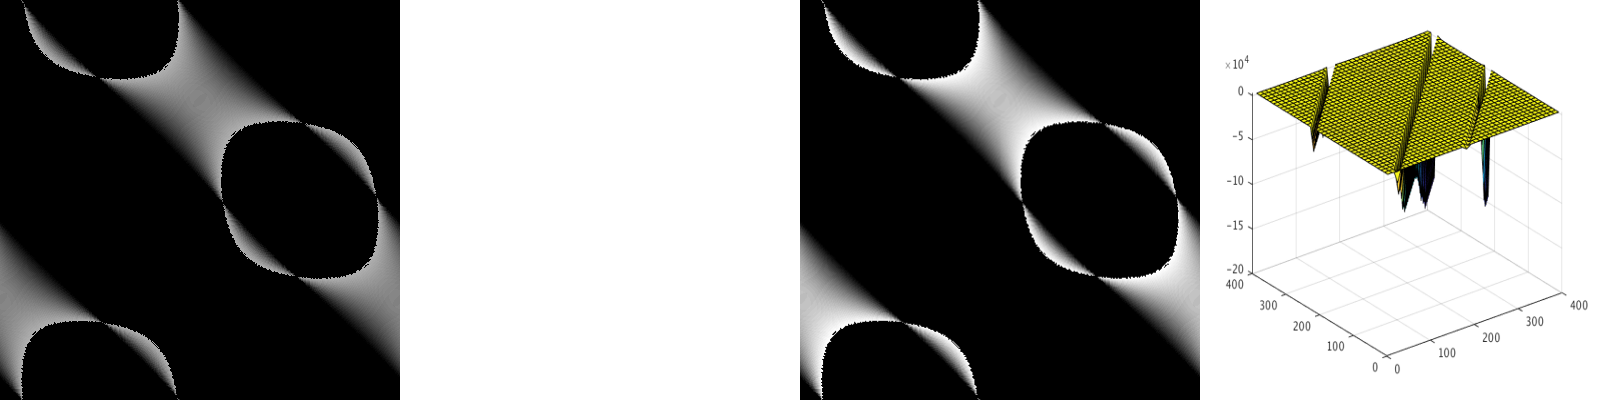
\includegraphics[width=160mm]{figs/q2_im2_bad3_all_figs.png}
	\caption{BAD ATTEMPT 3: Left: Unit normals with test light at (0, 0, 1). Center-left: 
        Recovered albedo. Center-right: Recovered normals with test light at (0, 
        0, 1) (Non-unit normals take albedo into account.) Right: Surface plot. 
        This was my last attempt at HLSE. I don't think it can be used for this 
        problem.}
\end{figure}

\subsection{The Fourth Attempt}

While our overall initial strategy of non-homogeneous least squared error seemed 
correct, there was a problem. The sum of the 
light intensities for each channel is not the same, but the method for solving 
photometric stereo assumes the same intensity of light for each of the different 
light locations. Therefore, we must multiply the image channels with less 
intensity by the inverse of their relative intensity to bring them up to the 
same level as the highest-intensity channel. This, again, assumes that lights 
are linear, since we are essentially summing up the intensities of the different 
lights. This yields the expected result and happens to handle the constraint of 
a constant, white albedo, as well.

\begin{figure}[!ht]
	\centering
	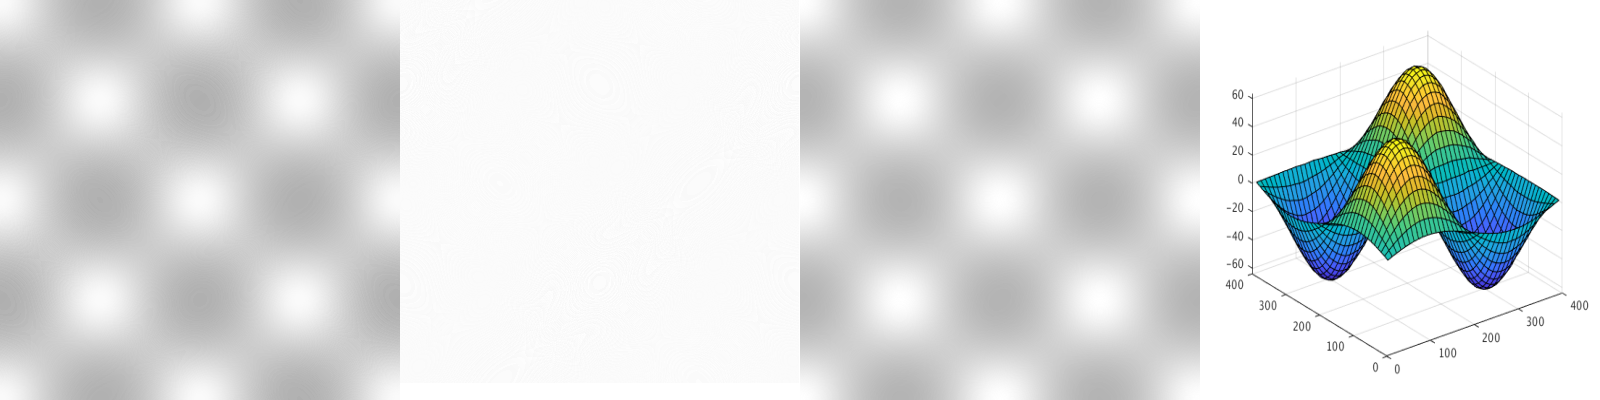
\includegraphics[width=160mm]{figs/q2_im2_good_all_figs.png}
	\caption{GOOD RESULT: Left: Unit normals with test light at (0, 0, 1). Center-left: 
        Recovered albedo. Center-right: Recovered normals with test light at (0, 
        0, 1) (Non-unit normals take albedo into account.) Right: Surface plot. 
        It looks correct to me!}
\end{figure}

And the other image:

\begin{figure}[!ht]
	\centering
	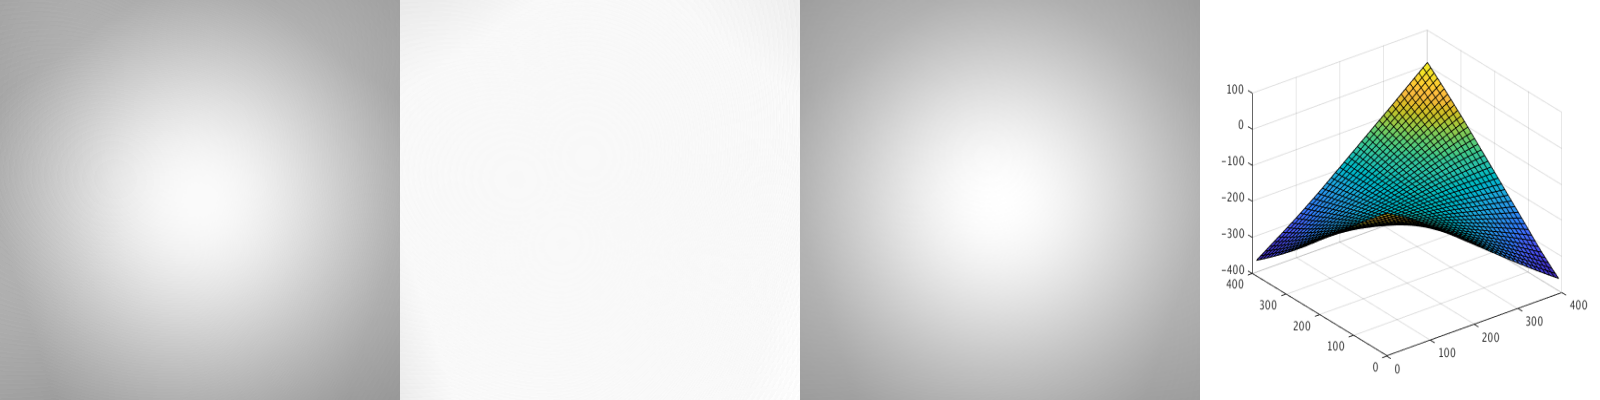
\includegraphics[width=160mm]{figs/q2_im1_good_all_figs.png}
	\caption{GOOD RESULT: Left: Unit normals with test light at (0, 0, 1). Center-left: 
        Recovered albedo. Center-right: Recovered normals with test light at (0, 
        0, 1) (Non-unit normals take albedo into account.) Right: Surface plot. 
        I expected this to be a hump with a local maximum at the center, but it 
        turns out that the surface has a saddle point in the middle instead. I 
        think this is just my intuition being wrong.}
\end{figure}

\section{Conclusion}

We have seen how easy it is to recover not only surface normals, but the surface 
proper given just a few lights (three or more) with the same intensity and known 
locations. We have also seen how these techniques can be applied to the slightly 
different problem of a single image with multiple lights with known intensities 
and locations by examinining each channel individually and finding 
corresponding pure red, pure green, and pure blue light position estimates. In 
this situation, we have shown that the homogeneous least squared method cannot 
be applied. However, the correct solution involved scaling each channel to 
account for the differences in light intensities.

\end{document}